\documentclass[twoside]{book}

% Packages required by doxygen
\usepackage{calc}
\usepackage{doxygen}
\usepackage{graphicx}
\usepackage[utf8]{inputenc}
\usepackage{makeidx}
\usepackage{multicol}
\usepackage{multirow}
\usepackage{textcomp}
\usepackage[table]{xcolor}

% NLS support packages
\usepackage{polski}
\usepackage[T1]{fontenc}

% Font selection
\usepackage[T1]{fontenc}
\usepackage{mathptmx}
\usepackage[scaled=.90]{helvet}
\usepackage{courier}
\usepackage{amssymb}
\usepackage{sectsty}
\renewcommand{\familydefault}{\sfdefault}
\allsectionsfont{%
  \fontseries{bc}\selectfont%
  \color{darkgray}%
}
\renewcommand{\DoxyLabelFont}{%
  \fontseries{bc}\selectfont%
  \color{darkgray}%
}

% Page & text layout
\usepackage{geometry}
\geometry{%
  a4paper,%
  top=2.5cm,%
  bottom=2.5cm,%
  left=2.5cm,%
  right=2.5cm%
}
\tolerance=750
\hfuzz=15pt
\hbadness=750
\setlength{\emergencystretch}{15pt}
\setlength{\parindent}{0cm}
\setlength{\parskip}{0.2cm}
\makeatletter
\renewcommand{\paragraph}{%
  \@startsection{paragraph}{4}{0ex}{-1.0ex}{1.0ex}{%
    \normalfont\normalsize\bfseries\SS@parafont%
  }%
}
\renewcommand{\subparagraph}{%
  \@startsection{subparagraph}{5}{0ex}{-1.0ex}{1.0ex}{%
    \normalfont\normalsize\bfseries\SS@subparafont%
  }%
}
\makeatother

% Headers & footers
\usepackage{fancyhdr}
\pagestyle{fancyplain}
\fancyhead[LE]{\fancyplain{}{\bfseries\thepage}}
\fancyhead[CE]{\fancyplain{}{}}
\fancyhead[RE]{\fancyplain{}{\bfseries\leftmark}}
\fancyhead[LO]{\fancyplain{}{\bfseries\rightmark}}
\fancyhead[CO]{\fancyplain{}{}}
\fancyhead[RO]{\fancyplain{}{\bfseries\thepage}}
\fancyfoot[LE]{\fancyplain{}{}}
\fancyfoot[CE]{\fancyplain{}{}}
\fancyfoot[RE]{\fancyplain{}{\bfseries\scriptsize Wygenerowano Śr, 11 mar 2015 23\-:03\-:37 dla lab1 programem Doxygen }}
\fancyfoot[LO]{\fancyplain{}{\bfseries\scriptsize Wygenerowano Śr, 11 mar 2015 23\-:03\-:37 dla lab1 programem Doxygen }}
\fancyfoot[CO]{\fancyplain{}{}}
\fancyfoot[RO]{\fancyplain{}{}}
\renewcommand{\footrulewidth}{0.4pt}
\renewcommand{\chaptermark}[1]{%
  \markboth{#1}{}%
}
\renewcommand{\sectionmark}[1]{%
  \markright{\thesection\ #1}%
}

% Indices & bibliography
\usepackage{natbib}
\usepackage[titles]{tocloft}
\setcounter{tocdepth}{3}
\setcounter{secnumdepth}{5}
\makeindex

% Hyperlinks (required, but should be loaded last)
\usepackage{ifpdf}
\ifpdf
  \usepackage[pdftex,pagebackref=true]{hyperref}
\else
  \usepackage[ps2pdf,pagebackref=true]{hyperref}
\fi
\hypersetup{%
  colorlinks=true,%
  linkcolor=blue,%
  citecolor=blue,%
  unicode%
}

% Custom commands
\newcommand{\clearemptydoublepage}{%
  \newpage{\pagestyle{empty}\cleardoublepage}%
}


%===== C O N T E N T S =====

\begin{document}

% Titlepage & ToC
\hypersetup{pageanchor=false}
\pagenumbering{roman}
\begin{titlepage}
\vspace*{7cm}
\begin{center}%
{\Large lab1 \\[1ex]\large 0.\-0001 }\\
\vspace*{1cm}
{\large Wygenerowano przez Doxygen 1.8.6}\\
\vspace*{0.5cm}
{\small Śr, 11 mar 2015 23:03:37}\\
\end{center}
\end{titlepage}
\clearemptydoublepage
\tableofcontents
\clearemptydoublepage
\pagenumbering{arabic}
\hypersetup{pageanchor=true}

%--- Begin generated contents ---
\chapter{lab1}
\label{index}\hypertarget{index}{}\begin{DoxyAuthor}{Autor}
Filip Malinowski 
\end{DoxyAuthor}
\begin{DoxyDate}{Data}
22.\-04.\-2015 
\end{DoxyDate}
\begin{DoxyVersion}{Wersja}
0.\-0005
\end{DoxyVersion}
Program sluzacy do uruchamiania algorytmow i badania ich szybkosci dzialania.\par
W programie zaimplementowane sa algorytmy\-:\par

\begin{DoxyItemize}
\item sortowania szybkiego stosu\par

\item sortowania szybkiego po optymalizacji pivot stosu\par

\item sortowania przez scalanie stosu\par

\item sortowania przez kopcowanie stosu
\end{DoxyItemize}

Do wykonania podanych powyzej trzech ostatnich algorytmow zostaly zaimplementowane potrzebne struktury danych (stos, kolejka, lista oraz lista tablicowa, lista asocjacyjna, tablica z haszowaniem).\par
\par
Ciala klas znajduja sie w folderze ./prj/inc\par
Definicje metod znajduja sie w folderze ./prj/src\par
Sprawozdanie znajduje sie w folderze ./prj/doc/sprawozdanie\par
\par
Format wywolania\-:\par

\begin{DoxyCode}
./prj/make clean\(\backslash\)n
./prj/make\(\backslash\)n
\end{DoxyCode}
 
\chapter{Indeks hierarchiczny}
\section{Hierarchia klas}
Ta lista dziedziczenia posortowana jest z grubsza, choć nie całkowicie, alfabetycznie\-:\begin{DoxyCompactList}
\item \contentsline{section}{Benchmark}{\pageref{class_benchmark}}{}
\begin{DoxyCompactList}
\item \contentsline{section}{Mnozenie}{\pageref{class_mnozenie}}{}
\end{DoxyCompactList}
\end{DoxyCompactList}

\chapter{Indeks klas}
\section{Lista klas}
Tutaj znajdują się klasy, struktury, unie i interfejsy wraz z ich krótkimi opisami\-:\begin{DoxyCompactList}
\item\contentsline{section}{\hyperlink{class_algorithm_kolejka}{Algorithm\-Kolejka} \\*Klasa \hyperlink{class_algorithm_kolejka}{Algorithm\-Kolejka} modelujaca algorytm wczytywania do kolejki. Obiekt tego typu reprezentuje algorytm wykonujacy wykonujacy wczytywanie zadanej ilosci elementow do kolejki }{\pageref{class_algorithm_kolejka}}{}
\item\contentsline{section}{\hyperlink{class_algorithm_lista}{Algorithm\-Lista} \\*Klasa \hyperlink{class_algorithm_lista}{Algorithm\-Lista} modelujaca algorytm wczytywania do kolejki. Obiekt tego typu reprezentuje algorytm wykonujacy wykonujacy wczytywanie zadanej ilosci elementow do listy }{\pageref{class_algorithm_lista}}{}
\item\contentsline{section}{\hyperlink{class_algorithm_stos}{Algorithm\-Stos} \\*Klasa \hyperlink{class_algorithm_stos}{Algorithm\-Stos} modelujaca algorytm wczytywania do stosu. Obiekt tego typu reprezentuje algorytm wykonujacy wykonujacy wczytywanie zadanej ilosci elementow do stosu }{\pageref{class_algorithm_stos}}{}
\item\contentsline{section}{\hyperlink{class_benchmark}{Benchmark} \\*Klasa \hyperlink{class_benchmark}{Benchmark} modelujaca program benchmarkujacy. Obiekt tego typu reprezentuje program sprawdzajacy szybkosc wykonywania algorytmow }{\pageref{class_benchmark}}{}
\item\contentsline{section}{\hyperlink{class_kolejka}{Kolejka} \\*Klasa \hyperlink{class_kolejka}{Kolejka} modelujaca strukture danych typu kolejka. Obiekt tego typu reprezentuje strukture danych typu kolejka wraz z operacjami mozliwymi do wykonania na tej strukturze }{\pageref{class_kolejka}}{}
\item\contentsline{section}{\hyperlink{struct_lista_1_1_komorka}{Lista\-::\-Komorka} \\*Struktura \hyperlink{struct_lista_1_1_komorka}{Komorka}. Obiekt tego typu reprezentuje pojedyncza komorke wraz ze wskaznikiem na nastepna komorke listy }{\pageref{struct_lista_1_1_komorka}}{}
\item\contentsline{section}{\hyperlink{class_lista}{Lista} \\*Klasa \hyperlink{class_lista}{Lista} modelujaca strukture danych typu lista. Obiekt tego typu reprezentuje strukture danych typu lista wraz z operacjami mozliwymi do wykonania na tej strukturze }{\pageref{class_lista}}{}
\item\contentsline{section}{\hyperlink{class_mnozenie}{Mnozenie} \\*Klasa \hyperlink{class_mnozenie}{Mnozenie} modelujaca algorytm mnozenia. Obiekt tego typu reprezentuje algorytm wykonujacy dzialanie mnozenia kazdego elementu tablicy tab przez 2 }{\pageref{class_mnozenie}}{}
\item\contentsline{section}{\hyperlink{class_stos}{Stos} \\*Klasa \hyperlink{class_stos}{Stos} modelujaca strukture danych typu stos. Obiekt tego typu reprezentuje strukture danych typu stos wraz z operacjami mozliwymi do wykonania na tej strukturze }{\pageref{class_stos}}{}
\end{DoxyCompactList}

\chapter{Indeks plików}
\section{Lista plików}
Tutaj znajduje się lista wszystkich plików z ich krótkimi opisami\-:\begin{DoxyCompactList}
\item\contentsline{section}{\hyperlink{algorithm2_8cpp}{algorithm2.\-cpp} }{\pageref{algorithm2_8cpp}}{}
\item\contentsline{section}{\hyperlink{algorithm2_8hh}{algorithm2.\-hh} }{\pageref{algorithm2_8hh}}{}
\item\contentsline{section}{\hyperlink{algorithm__kolejka_8cpp}{algorithm\-\_\-kolejka.\-cpp} }{\pageref{algorithm__kolejka_8cpp}}{}
\item\contentsline{section}{\hyperlink{algorithm__kolejka_8hh}{algorithm\-\_\-kolejka.\-hh} }{\pageref{algorithm__kolejka_8hh}}{}
\item\contentsline{section}{\hyperlink{algorithm__lista_8cpp}{algorithm\-\_\-lista.\-cpp} }{\pageref{algorithm__lista_8cpp}}{}
\item\contentsline{section}{\hyperlink{algorithm__lista_8hh}{algorithm\-\_\-lista.\-hh} }{\pageref{algorithm__lista_8hh}}{}
\item\contentsline{section}{\hyperlink{algorithm__stos_8cpp}{algorithm\-\_\-stos.\-cpp} }{\pageref{algorithm__stos_8cpp}}{}
\item\contentsline{section}{\hyperlink{algorithm__stos_8hh}{algorithm\-\_\-stos.\-hh} }{\pageref{algorithm__stos_8hh}}{}
\item\contentsline{section}{\hyperlink{benchmark_8cpp}{benchmark.\-cpp} }{\pageref{benchmark_8cpp}}{}
\item\contentsline{section}{\hyperlink{benchmark_8hh}{benchmark.\-hh} }{\pageref{benchmark_8hh}}{}
\item\contentsline{section}{\hyperlink{generate_8cpp}{generate.\-cpp} }{\pageref{generate_8cpp}}{}
\item\contentsline{section}{\hyperlink{kolejka_8cpp}{kolejka.\-cpp} }{\pageref{kolejka_8cpp}}{}
\item\contentsline{section}{\hyperlink{kolejka_8hh}{kolejka.\-hh} }{\pageref{kolejka_8hh}}{}
\item\contentsline{section}{\hyperlink{lista_8cpp}{lista.\-cpp} }{\pageref{lista_8cpp}}{}
\item\contentsline{section}{\hyperlink{lista_8hh}{lista.\-hh} }{\pageref{lista_8hh}}{}
\item\contentsline{section}{\hyperlink{main_8cpp}{main.\-cpp} }{\pageref{main_8cpp}}{}
\item\contentsline{section}{\hyperlink{stos_8cpp}{stos.\-cpp} }{\pageref{stos_8cpp}}{}
\item\contentsline{section}{\hyperlink{stos_8hh}{stos.\-hh} }{\pageref{stos_8hh}}{}
\item\contentsline{section}{\hyperlink{tab__lista_8cpp}{tab\-\_\-lista.\-cpp} }{\pageref{tab__lista_8cpp}}{}
\item\contentsline{section}{\hyperlink{tab__lista_8hh}{tab\-\_\-lista.\-hh} }{\pageref{tab__lista_8hh}}{}
\end{DoxyCompactList}

\chapter{Dokumentacja klas}
\hypertarget{class_benchmark}{\section{Dokumentacja klasy Benchmark}
\label{class_benchmark}\index{Benchmark@{Benchmark}}
}


Klasa \hyperlink{class_benchmark}{Benchmark} modelujaca program benchmarkujacy. Obiekt tego typu reprezentuje program sprawdzajacy szybkosc wykonywania algorytmow.  




{\ttfamily \#include $<$benchmark.\-hh$>$}



Diagram dziedziczenia dla Benchmark\nopagebreak
\begin{figure}[H]
\begin{center}
\leavevmode
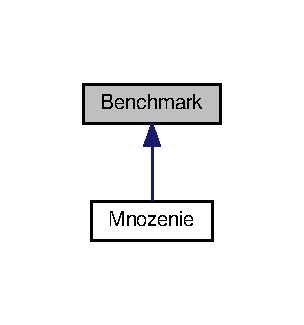
\includegraphics[width=350pt]{class_benchmark__inherit__graph}
\end{center}
\end{figure}
\subsection*{Metody publiczne}
\begin{DoxyCompactItemize}
\item 
\hyperlink{class_benchmark_acfca497989836a688d44477802e822d8}{Benchmark} ()
\begin{DoxyCompactList}\small\item\em Konstrukor obiektu \hyperlink{class_benchmark}{Benchmark}. \end{DoxyCompactList}\item 
\hyperlink{class_benchmark_a20476e07f09e2b20ed3e9a7f13a570e6}{$\sim$\-Benchmark} ()
\begin{DoxyCompactList}\small\item\em Destruktor obiektu \hyperlink{class_benchmark}{Benchmark}. \end{DoxyCompactList}\item 
virtual void \hyperlink{class_benchmark_a900bc0d26c2ed6aa45afe4d5b295ccd1}{test\-Algorithm} (\hyperlink{class_benchmark}{Benchmark} $\ast$\-\_\-algorithm, int \-\_\-n) const 
\begin{DoxyCompactList}\small\item\em Metoda testowania algorytmu. Metoda sluzy to testowania szybkosci dzialania algorytmu. Wykonuje testowany algorytm dla 5 kolejnych ilosci elementow. Wykonanie algorytmu dla danego zestawu liczb powtarza dwa razy i usrednia wynik. Otrzymany czas wraz z iloscia testowanych danych zapisuje w pliku ret\-\_\-data.\-txt. \end{DoxyCompactList}\item 
virtual void \hyperlink{class_benchmark_a6363894c058e8bfe146de09d7126b29c}{run\-Algorithm} (int \-\_\-border)
\begin{DoxyCompactList}\small\item\em Metoda uruchamiania algorytmu. Metoda sluzy do wykonywania danego algorytmu. W klasie \hyperlink{class_benchmark}{Benchmark} nie ma konkretnego dzialania. \end{DoxyCompactList}\end{DoxyCompactItemize}
\subsection*{Atrybuty prywatne}
\begin{DoxyCompactItemize}
\item 
std\-::string \hyperlink{class_benchmark_aee0beda65009e7334d34c5957f78c49a}{nazwy} \mbox{[}4\mbox{]} = \{\char`\"{}ret\-\_\-data1.\-txt\char`\"{}, \char`\"{}ret\-\_\-data2.\-txt\char`\"{}, \char`\"{}ret\-\_\-data3.\-txt\char`\"{}, \char`\"{}ret\-\_\-data4.\-txt\char`\"{}\}
\begin{DoxyCompactList}\small\item\em Tablica stringow przechowujaca nazwy plikow do zapisu. \end{DoxyCompactList}\end{DoxyCompactItemize}


\subsection{Opis szczegółowy}


Definicja w linii 11 pliku benchmark.\-hh.



\subsection{Dokumentacja konstruktora i destruktora}
\hypertarget{class_benchmark_acfca497989836a688d44477802e822d8}{\index{Benchmark@{Benchmark}!Benchmark@{Benchmark}}
\index{Benchmark@{Benchmark}!Benchmark@{Benchmark}}
\subsubsection[{Benchmark}]{\setlength{\rightskip}{0pt plus 5cm}Benchmark\-::\-Benchmark (
\begin{DoxyParamCaption}
{}
\end{DoxyParamCaption}
)\hspace{0.3cm}{\ttfamily [inline]}}}\label{class_benchmark_acfca497989836a688d44477802e822d8}


Definicja w linii 23 pliku benchmark.\-hh.

\hypertarget{class_benchmark_a20476e07f09e2b20ed3e9a7f13a570e6}{\index{Benchmark@{Benchmark}!$\sim$\-Benchmark@{$\sim$\-Benchmark}}
\index{$\sim$\-Benchmark@{$\sim$\-Benchmark}!Benchmark@{Benchmark}}
\subsubsection[{$\sim$\-Benchmark}]{\setlength{\rightskip}{0pt plus 5cm}Benchmark\-::$\sim$\-Benchmark (
\begin{DoxyParamCaption}
{}
\end{DoxyParamCaption}
)\hspace{0.3cm}{\ttfamily [inline]}}}\label{class_benchmark_a20476e07f09e2b20ed3e9a7f13a570e6}


Definicja w linii 28 pliku benchmark.\-hh.



\subsection{Dokumentacja funkcji składowych}
\hypertarget{class_benchmark_a6363894c058e8bfe146de09d7126b29c}{\index{Benchmark@{Benchmark}!run\-Algorithm@{run\-Algorithm}}
\index{run\-Algorithm@{run\-Algorithm}!Benchmark@{Benchmark}}
\subsubsection[{run\-Algorithm}]{\setlength{\rightskip}{0pt plus 5cm}virtual void Benchmark\-::run\-Algorithm (
\begin{DoxyParamCaption}
\item[{int}]{\-\_\-border}
\end{DoxyParamCaption}
)\hspace{0.3cm}{\ttfamily [inline]}, {\ttfamily [virtual]}}}\label{class_benchmark_a6363894c058e8bfe146de09d7126b29c}

\begin{DoxyParams}[1]{Parametry}
\mbox{\tt in}  & {\em \-\_\-border} & -\/ ilosc elementow dla ktorych algorytm ma wykonac swoje dzialanie. \\
\hline
\end{DoxyParams}


Reimplementowana w \hyperlink{class_algorithm2_a409e58d5fb0b6d2407cc986cf163703b}{Algorithm2}, \hyperlink{class_algorithm_kolejka_ae9da3f1862fd90feb4a3c1d6b4f3dd8d}{Algorithm\-Kolejka}, \hyperlink{class_algorithm_lista_a5c41dbbd3ae7a9ac34edec1a51bc8eb1}{Algorithm\-Lista} i \hyperlink{class_algorithm_stos_a889f7150ae3651b40e5acca7542dbbd1}{Algorithm\-Stos}.



Definicja w linii 48 pliku benchmark.\-hh.



Oto graf wywoływań tej funkcji\-:\nopagebreak
\begin{figure}[H]
\begin{center}
\leavevmode
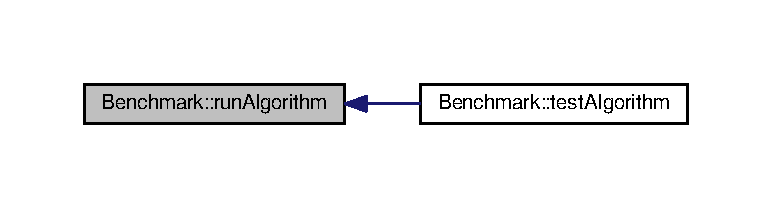
\includegraphics[width=350pt]{class_benchmark_a6363894c058e8bfe146de09d7126b29c_icgraph}
\end{center}
\end{figure}


\hypertarget{class_benchmark_a900bc0d26c2ed6aa45afe4d5b295ccd1}{\index{Benchmark@{Benchmark}!test\-Algorithm@{test\-Algorithm}}
\index{test\-Algorithm@{test\-Algorithm}!Benchmark@{Benchmark}}
\subsubsection[{test\-Algorithm}]{\setlength{\rightskip}{0pt plus 5cm}void Benchmark\-::test\-Algorithm (
\begin{DoxyParamCaption}
\item[{{\bf Benchmark} $\ast$}]{\-\_\-algorithm, }
\item[{int}]{\-\_\-n}
\end{DoxyParamCaption}
) const\hspace{0.3cm}{\ttfamily [virtual]}}}\label{class_benchmark_a900bc0d26c2ed6aa45afe4d5b295ccd1}

\begin{DoxyParams}[1]{Parametry}
\mbox{\tt in}  & {\em \-\_\-algorithm} & -\/ testowany algorytm. \\
\hline
\mbox{\tt in}  & {\em \-\_\-n} & -\/ indeks nazwy pliku \\
\hline
\end{DoxyParams}


Definicja w linii 12 pliku benchmark.\-cpp.



Oto graf wywołań dla tej funkcji\-:\nopagebreak
\begin{figure}[H]
\begin{center}
\leavevmode
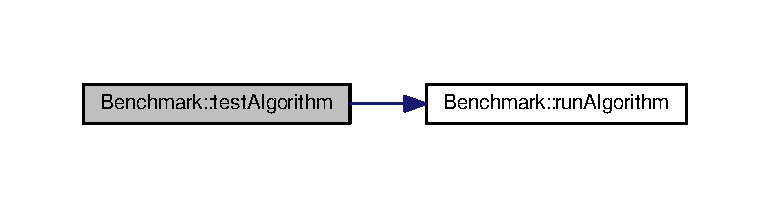
\includegraphics[width=350pt]{class_benchmark_a900bc0d26c2ed6aa45afe4d5b295ccd1_cgraph}
\end{center}
\end{figure}




\subsection{Dokumentacja atrybutów składowych}
\hypertarget{class_benchmark_aee0beda65009e7334d34c5957f78c49a}{\index{Benchmark@{Benchmark}!nazwy@{nazwy}}
\index{nazwy@{nazwy}!Benchmark@{Benchmark}}
\subsubsection[{nazwy}]{\setlength{\rightskip}{0pt plus 5cm}std\-::string Benchmark\-::nazwy\mbox{[}4\mbox{]} = \{\char`\"{}ret\-\_\-data1.\-txt\char`\"{}, \char`\"{}ret\-\_\-data2.\-txt\char`\"{}, \char`\"{}ret\-\_\-data3.\-txt\char`\"{}, \char`\"{}ret\-\_\-data4.\-txt\char`\"{}\}\hspace{0.3cm}{\ttfamily [private]}}}\label{class_benchmark_aee0beda65009e7334d34c5957f78c49a}


Definicja w linii 16 pliku benchmark.\-hh.



Dokumentacja dla tej klasy została wygenerowana z plików\-:\begin{DoxyCompactItemize}
\item 
\hyperlink{benchmark_8hh}{benchmark.\-hh}\item 
\hyperlink{benchmark_8cpp}{benchmark.\-cpp}\end{DoxyCompactItemize}

\hypertarget{class_mnozenie}{\section{Dokumentacja klasy Mnozenie}
\label{class_mnozenie}\index{Mnozenie@{Mnozenie}}
}


Klasa \hyperlink{class_mnozenie}{Mnozenie} modelujaca algorytm potegowania. Obiekt tego typu reprezentuje algorytm wykonujacy dzialanie mnozenia kazdego elementu tablicy tab przez 2.  




{\ttfamily \#include $<$algorithm1.\-hh$>$}



Diagram dziedziczenia dla Mnozenie\nopagebreak
\begin{figure}[H]
\begin{center}
\leavevmode
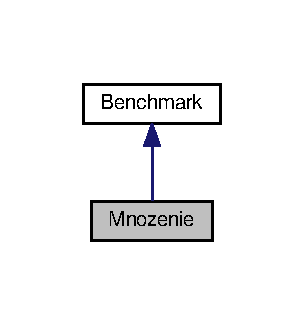
\includegraphics[width=146pt]{class_mnozenie__inherit__graph}
\end{center}
\end{figure}


Diagram współpracy dla Mnozenie\-:\nopagebreak
\begin{figure}[H]
\begin{center}
\leavevmode
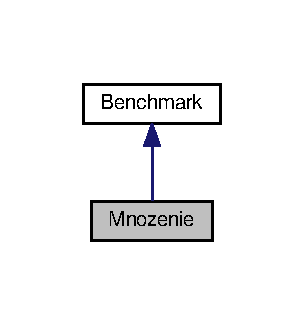
\includegraphics[width=146pt]{class_mnozenie__coll__graph}
\end{center}
\end{figure}
\subsection*{Metody publiczne}
\begin{DoxyCompactItemize}
\item 
\hyperlink{class_mnozenie_aac38391baa7ffd14970526902ab750de}{Mnozenie} ()
\begin{DoxyCompactList}\small\item\em Konstruktor obiektu \hyperlink{class_mnozenie}{Mnozenie}. \end{DoxyCompactList}\item 
\hyperlink{class_mnozenie_a5252eb846883e6813fc2fef82a30c751}{Mnozenie} (int \-\_\-tab\mbox{[}\hyperlink{benchmark_8hh_a70ed59adcb4159ac551058053e649640}{S\-I\-Z\-E}\mbox{]})
\begin{DoxyCompactList}\small\item\em Konstruktor parametryczny obiektu \hyperlink{class_mnozenie}{Mnozenie}. \end{DoxyCompactList}\item 
\hyperlink{class_mnozenie_ad57f03bc66770fb6a442169781ee2156}{$\sim$\-Mnozenie} ()
\begin{DoxyCompactList}\small\item\em Destruktor obiektu \hyperlink{class_mnozenie}{Mnozenie}. \end{DoxyCompactList}\item 
virtual void \hyperlink{class_mnozenie_a039792aaa5ce9723cd61d29869cf0101}{test\-Algorithm} (\hyperlink{class_benchmark}{Benchmark} $\ast$\-\_\-algorithm)
\begin{DoxyCompactList}\small\item\em Metoda testowania algorytmu. Metoda sluzy do testowania szybkosci dzialania algorytmu. W klasie \hyperlink{class_mnozenie}{Mnozenie} nie ma konkretnego dzialania. \end{DoxyCompactList}\item 
virtual void \hyperlink{class_mnozenie_a46b1c55b7ba208fa137065147e107be9}{run\-Algorithm} (int \-\_\-border)
\begin{DoxyCompactList}\small\item\em Metoda uruchamiania algorytmu. Metoda sluzy to wykonywania danego algorytmu. Mnozy kazdy element tablicy przez liczbe 2. \end{DoxyCompactList}\end{DoxyCompactItemize}
\subsection*{Atrybuty prywatne}
\begin{DoxyCompactItemize}
\item 
int \hyperlink{class_mnozenie_a6dc67671f84a557d97c322b8af528359}{tab} \mbox{[}\hyperlink{benchmark_8hh_a70ed59adcb4159ac551058053e649640}{S\-I\-Z\-E}\mbox{]}
\end{DoxyCompactItemize}


\subsection{Opis szczegółowy}


Definicja w linii 9 pliku algorithm1.\-hh.



\subsection{Dokumentacja konstruktora i destruktora}
\hypertarget{class_mnozenie_aac38391baa7ffd14970526902ab750de}{\index{Mnozenie@{Mnozenie}!Mnozenie@{Mnozenie}}
\index{Mnozenie@{Mnozenie}!Mnozenie@{Mnozenie}}
\subsubsection[{Mnozenie}]{\setlength{\rightskip}{0pt plus 5cm}Mnozenie\-::\-Mnozenie (
\begin{DoxyParamCaption}
{}
\end{DoxyParamCaption}
)\hspace{0.3cm}{\ttfamily [inline]}}}\label{class_mnozenie_aac38391baa7ffd14970526902ab750de}


Definicja w linii 17 pliku algorithm1.\-hh.

\hypertarget{class_mnozenie_a5252eb846883e6813fc2fef82a30c751}{\index{Mnozenie@{Mnozenie}!Mnozenie@{Mnozenie}}
\index{Mnozenie@{Mnozenie}!Mnozenie@{Mnozenie}}
\subsubsection[{Mnozenie}]{\setlength{\rightskip}{0pt plus 5cm}Mnozenie\-::\-Mnozenie (
\begin{DoxyParamCaption}
\item[{int}]{\-\_\-tab\mbox{[}\-S\-I\-Z\-E\mbox{]}}
\end{DoxyParamCaption}
)\hspace{0.3cm}{\ttfamily [inline]}}}\label{class_mnozenie_a5252eb846883e6813fc2fef82a30c751}

\begin{DoxyParams}[1]{Parametry}
\mbox{\tt in}  & {\em \-\_\-tab} & -\/ tablica przechowujaca dane wejsciowe. \\
\hline
\end{DoxyParams}


Definicja w linii 23 pliku algorithm1.\-hh.

\hypertarget{class_mnozenie_ad57f03bc66770fb6a442169781ee2156}{\index{Mnozenie@{Mnozenie}!$\sim$\-Mnozenie@{$\sim$\-Mnozenie}}
\index{$\sim$\-Mnozenie@{$\sim$\-Mnozenie}!Mnozenie@{Mnozenie}}
\subsubsection[{$\sim$\-Mnozenie}]{\setlength{\rightskip}{0pt plus 5cm}Mnozenie\-::$\sim$\-Mnozenie (
\begin{DoxyParamCaption}
{}
\end{DoxyParamCaption}
)\hspace{0.3cm}{\ttfamily [inline]}}}\label{class_mnozenie_ad57f03bc66770fb6a442169781ee2156}


Definicja w linii 28 pliku algorithm1.\-hh.



\subsection{Dokumentacja funkcji składowych}
\hypertarget{class_mnozenie_a46b1c55b7ba208fa137065147e107be9}{\index{Mnozenie@{Mnozenie}!run\-Algorithm@{run\-Algorithm}}
\index{run\-Algorithm@{run\-Algorithm}!Mnozenie@{Mnozenie}}
\subsubsection[{run\-Algorithm}]{\setlength{\rightskip}{0pt plus 5cm}void Mnozenie\-::run\-Algorithm (
\begin{DoxyParamCaption}
\item[{int}]{\-\_\-border}
\end{DoxyParamCaption}
)\hspace{0.3cm}{\ttfamily [virtual]}}}\label{class_mnozenie_a46b1c55b7ba208fa137065147e107be9}

\begin{DoxyParams}[1]{Parametry}
\mbox{\tt in}  & {\em \-\_\-border} & -\/ ilosc elementow dla ktorych algorytm ma wykonac swoje dzialanie. \\
\hline
\end{DoxyParams}


Reimplementowana z \hyperlink{class_benchmark_a6363894c058e8bfe146de09d7126b29c}{Benchmark}.



Definicja w linii 7 pliku algorithm1.\-cpp.

\hypertarget{class_mnozenie_a039792aaa5ce9723cd61d29869cf0101}{\index{Mnozenie@{Mnozenie}!test\-Algorithm@{test\-Algorithm}}
\index{test\-Algorithm@{test\-Algorithm}!Mnozenie@{Mnozenie}}
\subsubsection[{test\-Algorithm}]{\setlength{\rightskip}{0pt plus 5cm}virtual void Mnozenie\-::test\-Algorithm (
\begin{DoxyParamCaption}
\item[{{\bf Benchmark} $\ast$}]{\-\_\-algorithm}
\end{DoxyParamCaption}
)\hspace{0.3cm}{\ttfamily [inline]}, {\ttfamily [virtual]}}}\label{class_mnozenie_a039792aaa5ce9723cd61d29869cf0101}

\begin{DoxyParams}[1]{Parametry}
\mbox{\tt in}  & {\em \-\_\-algorithm} & -\/ testowany algorytm. \\
\hline
\end{DoxyParams}


Definicja w linii 36 pliku algorithm1.\-hh.



\subsection{Dokumentacja atrybutów składowych}
\hypertarget{class_mnozenie_a6dc67671f84a557d97c322b8af528359}{\index{Mnozenie@{Mnozenie}!tab@{tab}}
\index{tab@{tab}!Mnozenie@{Mnozenie}}
\subsubsection[{tab}]{\setlength{\rightskip}{0pt plus 5cm}int Mnozenie\-::tab\mbox{[}{\bf S\-I\-Z\-E}\mbox{]}\hspace{0.3cm}{\ttfamily [private]}}}\label{class_mnozenie_a6dc67671f84a557d97c322b8af528359}


Definicja w linii 11 pliku algorithm1.\-hh.



Dokumentacja dla tej klasy została wygenerowana z plików\-:\begin{DoxyCompactItemize}
\item 
\hyperlink{algorithm1_8hh}{algorithm1.\-hh}\item 
\hyperlink{algorithm1_8cpp}{algorithm1.\-cpp}\end{DoxyCompactItemize}

\chapter{Dokumentacja plików}
\hypertarget{algorithm1_8cpp}{\section{Dokumentacja pliku algorithm1.\-cpp}
\label{algorithm1_8cpp}\index{algorithm1.\-cpp@{algorithm1.\-cpp}}
}
{\ttfamily \#include $<$iostream$>$}\\*
{\ttfamily \#include \char`\"{}benchmark.\-hh\char`\"{}}\\*
{\ttfamily \#include \char`\"{}algorithm1.\-hh\char`\"{}}\\*
Wykres zależności załączania dla algorithm1.\-cpp\-:\nopagebreak
\begin{figure}[H]
\begin{center}
\leavevmode
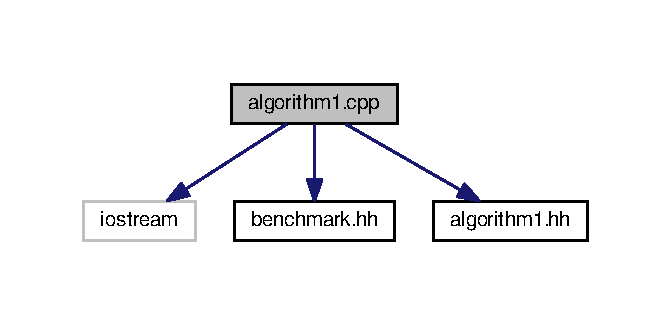
\includegraphics[width=322pt]{algorithm1_8cpp__incl}
\end{center}
\end{figure}

\hypertarget{algorithm1_8hh}{\section{Dokumentacja pliku algorithm1.\-hh}
\label{algorithm1_8hh}\index{algorithm1.\-hh@{algorithm1.\-hh}}
}
Ten wykres pokazuje, które pliki bezpośrednio lub pośrednio załączają ten plik\-:\nopagebreak
\begin{figure}[H]
\begin{center}
\leavevmode
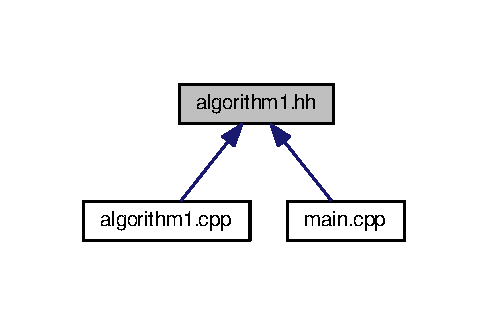
\includegraphics[width=234pt]{algorithm1_8hh__dep__incl}
\end{center}
\end{figure}
\subsection*{Komponenty}
\begin{DoxyCompactItemize}
\item 
class \hyperlink{class_algorithm1}{Algorithm1}
\begin{DoxyCompactList}\small\item\em Klasa \hyperlink{class_algorithm1}{Algorithm1} modelujaca algorytm sortowania stosu. Obiekt tego typu reprezentuje algorytm wykonujacy sortowanie szybkie na elementach stosu. Dziedziczy po klasie \hyperlink{class_benchmark}{Benchmark}. \end{DoxyCompactList}\end{DoxyCompactItemize}

\hypertarget{benchmark_8cpp}{\section{Dokumentacja pliku benchmark.\-cpp}
\label{benchmark_8cpp}\index{benchmark.\-cpp@{benchmark.\-cpp}}
}
{\ttfamily \#include $<$iostream$>$}\\*
{\ttfamily \#include $<$fstream$>$}\\*
{\ttfamily \#include $<$chrono$>$}\\*
{\ttfamily \#include \char`\"{}benchmark.\-hh\char`\"{}}\\*
Wykres zależności załączania dla benchmark.\-cpp\-:\nopagebreak
\begin{figure}[H]
\begin{center}
\leavevmode
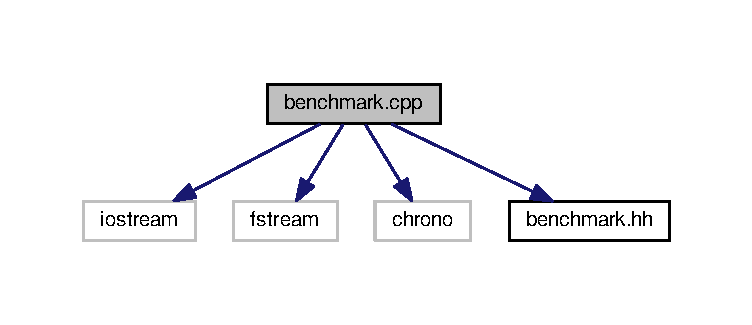
\includegraphics[width=350pt]{benchmark_8cpp__incl}
\end{center}
\end{figure}
\subsection*{Definicje}
\begin{DoxyCompactItemize}
\item 
\#define \hyperlink{benchmark_8cpp_a30362161c93e3f1a4ee4c673f535b5a8}{L\-E\-N\-G\-T\-H}~8
\item 
\#define \hyperlink{benchmark_8cpp_a96de703b1d261e201a5cbb65b4590f89}{R\-E\-P\-E\-A\-T\-S}~3
\end{DoxyCompactItemize}


\subsection{Dokumentacja definicji}
\hypertarget{benchmark_8cpp_a30362161c93e3f1a4ee4c673f535b5a8}{\index{benchmark.\-cpp@{benchmark.\-cpp}!L\-E\-N\-G\-T\-H@{L\-E\-N\-G\-T\-H}}
\index{L\-E\-N\-G\-T\-H@{L\-E\-N\-G\-T\-H}!benchmark.cpp@{benchmark.\-cpp}}
\subsubsection[{L\-E\-N\-G\-T\-H}]{\setlength{\rightskip}{0pt plus 5cm}\#define L\-E\-N\-G\-T\-H~8}}\label{benchmark_8cpp_a30362161c93e3f1a4ee4c673f535b5a8}


Definicja w linii 7 pliku benchmark.\-cpp.

\hypertarget{benchmark_8cpp_a96de703b1d261e201a5cbb65b4590f89}{\index{benchmark.\-cpp@{benchmark.\-cpp}!R\-E\-P\-E\-A\-T\-S@{R\-E\-P\-E\-A\-T\-S}}
\index{R\-E\-P\-E\-A\-T\-S@{R\-E\-P\-E\-A\-T\-S}!benchmark.cpp@{benchmark.\-cpp}}
\subsubsection[{R\-E\-P\-E\-A\-T\-S}]{\setlength{\rightskip}{0pt plus 5cm}\#define R\-E\-P\-E\-A\-T\-S~3}}\label{benchmark_8cpp_a96de703b1d261e201a5cbb65b4590f89}


Definicja w linii 8 pliku benchmark.\-cpp.


\hypertarget{benchmark_8hh}{\section{Dokumentacja pliku benchmark.\-hh}
\label{benchmark_8hh}\index{benchmark.\-hh@{benchmark.\-hh}}
}
Ten wykres pokazuje, które pliki bezpośrednio lub pośrednio załączają ten plik\-:\nopagebreak
\begin{figure}[H]
\begin{center}
\leavevmode
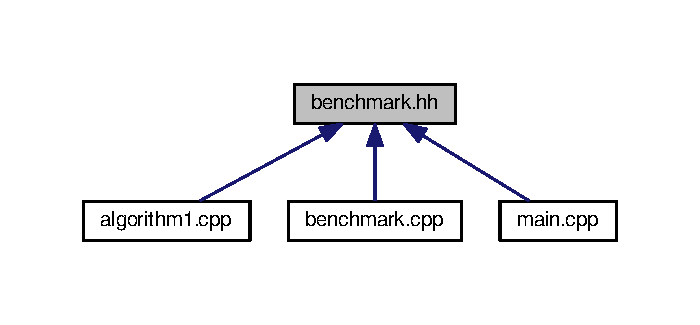
\includegraphics[width=350pt]{benchmark_8hh__dep__incl}
\end{center}
\end{figure}
\subsection*{Komponenty}
\begin{DoxyCompactItemize}
\item 
class \hyperlink{class_benchmark}{Benchmark}
\begin{DoxyCompactList}\small\item\em Klasa \hyperlink{class_benchmark}{Benchmark} modelujaca program benchmarkujacy. Obiekt tego typu reprezentuje program sprawdzajacy szybkosc wykonywania algorytmow. Dziedziczy po klasie \hyperlink{class_subject}{Subject}. \end{DoxyCompactList}\end{DoxyCompactItemize}
\subsection*{Definicje}
\begin{DoxyCompactItemize}
\item 
\#define \hyperlink{benchmark_8hh_a70ed59adcb4159ac551058053e649640}{S\-I\-Z\-E}~100000
\end{DoxyCompactItemize}


\subsection{Dokumentacja definicji}
\hypertarget{benchmark_8hh_a70ed59adcb4159ac551058053e649640}{\index{benchmark.\-hh@{benchmark.\-hh}!S\-I\-Z\-E@{S\-I\-Z\-E}}
\index{S\-I\-Z\-E@{S\-I\-Z\-E}!benchmark.hh@{benchmark.\-hh}}
\subsubsection[{S\-I\-Z\-E}]{\setlength{\rightskip}{0pt plus 5cm}\#define S\-I\-Z\-E~100000}}\label{benchmark_8hh_a70ed59adcb4159ac551058053e649640}


Definicja w linii 4 pliku benchmark.\-hh.


\hypertarget{generate_8cpp}{\section{Dokumentacja pliku generate.\-cpp}
\label{generate_8cpp}\index{generate.\-cpp@{generate.\-cpp}}
}
{\ttfamily \#include $<$fstream$>$}\\*
{\ttfamily \#include $<$iostream$>$}\\*
{\ttfamily \#include $<$cstdlib$>$}\\*
Wykres zależności załączania dla generate.\-cpp\-:\nopagebreak
\begin{figure}[H]
\begin{center}
\leavevmode
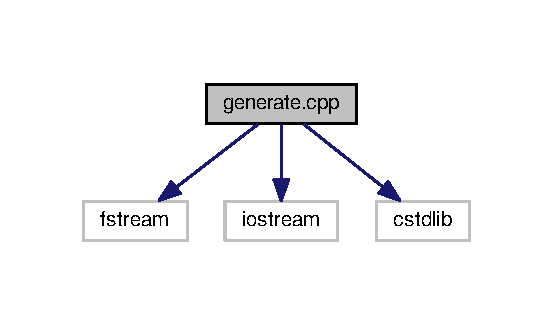
\includegraphics[width=265pt]{generate_8cpp__incl}
\end{center}
\end{figure}
\subsection*{Definicje}
\begin{DoxyCompactItemize}
\item 
\#define \hyperlink{generate_8cpp_a70ed59adcb4159ac551058053e649640}{S\-I\-Z\-E}~10000000
\end{DoxyCompactItemize}
\subsection*{Funkcje}
\begin{DoxyCompactItemize}
\item 
int \hyperlink{generate_8cpp_ae66f6b31b5ad750f1fe042a706a4e3d4}{main} ()
\begin{DoxyCompactList}\small\item\em Funkcja generowania pliku z danymi wejsciowymi. Generuje liczby losowe od 1 do 51 i zapisuje je do pliku o nazwie data.\-txt. \end{DoxyCompactList}\end{DoxyCompactItemize}


\subsection{Dokumentacja definicji}
\hypertarget{generate_8cpp_a70ed59adcb4159ac551058053e649640}{\index{generate.\-cpp@{generate.\-cpp}!S\-I\-Z\-E@{S\-I\-Z\-E}}
\index{S\-I\-Z\-E@{S\-I\-Z\-E}!generate.cpp@{generate.\-cpp}}
\subsubsection[{S\-I\-Z\-E}]{\setlength{\rightskip}{0pt plus 5cm}\#define S\-I\-Z\-E~10000000}}\label{generate_8cpp_a70ed59adcb4159ac551058053e649640}


Definicja w linii 5 pliku generate.\-cpp.



\subsection{Dokumentacja funkcji}
\hypertarget{generate_8cpp_ae66f6b31b5ad750f1fe042a706a4e3d4}{\index{generate.\-cpp@{generate.\-cpp}!main@{main}}
\index{main@{main}!generate.cpp@{generate.\-cpp}}
\subsubsection[{main}]{\setlength{\rightskip}{0pt plus 5cm}int main (
\begin{DoxyParamCaption}
{}
\end{DoxyParamCaption}
)}}\label{generate_8cpp_ae66f6b31b5ad750f1fe042a706a4e3d4}

\begin{DoxyRetVals}{Zwracane wartości}
{\em 0} & -\/ gdy funkcja zadziala poprawnie. \\
\hline
{\em 1} & -\/ gdy wystapi blad otwarcia pliku do zapisu. \\
\hline
\end{DoxyRetVals}


Definicja w linii 14 pliku generate.\-cpp.


\hypertarget{main_8cpp}{\section{Dokumentacja pliku main.\-cpp}
\label{main_8cpp}\index{main.\-cpp@{main.\-cpp}}
}
{\ttfamily \#include $<$iostream$>$}\\*
{\ttfamily \#include \char`\"{}observer.\-hh\char`\"{}}\\*
{\ttfamily \#include \char`\"{}subject.\-hh\char`\"{}}\\*
{\ttfamily \#include \char`\"{}benchmark.\-hh\char`\"{}}\\*
{\ttfamily \#include \char`\"{}writing\-\_\-observer.\-hh\char`\"{}}\\*
{\ttfamily \#include \char`\"{}tablicowe.\-hh\char`\"{}}\\*
{\ttfamily \#include \char`\"{}sort.\-hh\char`\"{}}\\*
{\ttfamily \#include \char`\"{}stos.\-hh\char`\"{}}\\*
{\ttfamily \#include \char`\"{}kolejka.\-hh\char`\"{}}\\*
{\ttfamily \#include \char`\"{}lista.\-hh\char`\"{}}\\*
{\ttfamily \#include \char`\"{}tab\-\_\-lista.\-hh\char`\"{}}\\*
{\ttfamily \#include \char`\"{}asocjacyjna.\-hh\char`\"{}}\\*
{\ttfamily \#include \char`\"{}mieszajaca.\-hh\char`\"{}}\\*
{\ttfamily \#include \char`\"{}binary\-\_\-tree.\-hh\char`\"{}}\\*
{\ttfamily \#include \char`\"{}rb\-\_\-tree.\-hh\char`\"{}}\\*
{\ttfamily \#include \char`\"{}algorithm1.\-hh\char`\"{}}\\*
{\ttfamily \#include \char`\"{}algorithm2.\-hh\char`\"{}}\\*
{\ttfamily \#include \char`\"{}algorithm3.\-hh\char`\"{}}\\*
{\ttfamily \#include \char`\"{}algorithm4.\-hh\char`\"{}}\\*
Wykres zależności załączania dla main.\-cpp\-:
\nopagebreak
\begin{figure}[H]
\begin{center}
\leavevmode
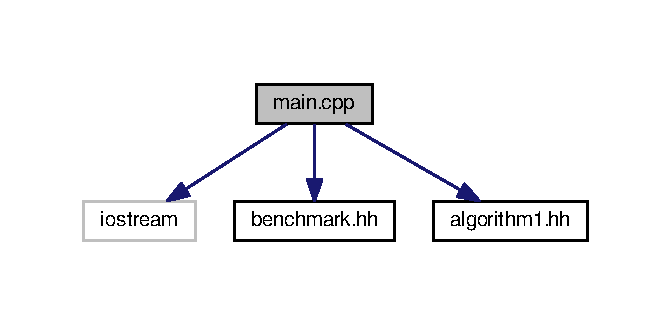
\includegraphics[width=350pt]{main_8cpp__incl}
\end{center}
\end{figure}
\subsection*{Funkcje}
\begin{DoxyCompactItemize}
\item 
int \hyperlink{main_8cpp_ae66f6b31b5ad750f1fe042a706a4e3d4}{main} ()
\begin{DoxyCompactList}\small\item\em Funkcja tworzaca i testujaca algorytm. Wczytuje dane otrzymane na strumien wejsciowy do tablicy data\mbox{[}\mbox{]}. Nastepnie tworzy obiekt \hyperlink{class_benchmark}{Benchmark} oraz obiekt Potegowanie. Pozniej uruchamia metode testujaca w obiekcie klasy \hyperlink{class_benchmark}{Benchmark} dla obiektu klasy Potegowanie. \end{DoxyCompactList}\end{DoxyCompactItemize}


\subsection{Dokumentacja funkcji}
\hypertarget{main_8cpp_ae66f6b31b5ad750f1fe042a706a4e3d4}{\index{main.\-cpp@{main.\-cpp}!main@{main}}
\index{main@{main}!main.cpp@{main.\-cpp}}
\subsubsection[{main}]{\setlength{\rightskip}{0pt plus 5cm}int main (
\begin{DoxyParamCaption}
{}
\end{DoxyParamCaption}
)}}\label{main_8cpp_ae66f6b31b5ad750f1fe042a706a4e3d4}

\begin{DoxyRetVals}{Zwracane wartości}
{\em 0} & -\/ domyslna wartosc zwracana przez funkcje. \\
\hline
\end{DoxyRetVals}


Definicja w linii 30 pliku main.\-cpp.


\hypertarget{strona-glowna_8dox}{\section{Dokumentacja pliku strona-\/glowna.dox}
\label{strona-glowna_8dox}\index{strona-\/glowna.\-dox@{strona-\/glowna.\-dox}}
}

%--- End generated contents ---

% Index
\newpage
\phantomsection
\addcontentsline{toc}{chapter}{Indeks}
\printindex

\end{document}
